\documentclass[../main.tex]{subfiles}
\graphicspath{{\subfix{../images/}}}
\begin{document}
\chapter{Related work}
\section{Recent relevant literature review}
\subsection{ Electric circuit education literature review}

This section provides a review of the literature relating to electric circuit education, how it is and how it can be improved.
\subsubsection{A Case Study for Comparing the Effectiveness of a Computer Simulation and a Hands-On Activity on Learning Electric Circuits. (Ekmekci, A., and Gulacar, O., 2015)
}

\subsubsection*{\underline{Methodology:}}

\begin{enumerate}
    \item Researchers would gather the students’ answer to the test a week prior to the day on which the study was to be conducted.
    \item On the day of the study, students would be divided into two groups, the students in the first group would be given a collection of circuit components, while the other group were told to use a circuit simulation program installed on their computers.
    \item Both groups were then given a lesson about circuits to further enhance their knowledge about the subject.
    \item After the lesson, students were tested once again, to measure the impact of their understanding and compare the differences between effectiveness of both hands-on and simulation learning experiences. 
\end{enumerate}
\subsubsection*{\underline{The results}} 

\begin{table}[h!]
    \caption{table showing the results of a test before a study (Maximum possible score: 8 )}  
    \centering
    \begin{tabular}{|c|c|c|c|c|c|}
       \hline
         & n & Mean & S.D & Lower & Upper \\
       \hline
       Computer-based & 16 & 4.38 & 1.45 & 3.69 & 5.08 \\
      \hline
       Hands-on & 20 & 5.20 & 1.44 & 4.44 & 5.80 \\
       \hline
       \end{tabular}
    \label{tab:1}
\end{table}
\begin{table}[!ht]
    \caption{ table showing the results of a test at the end of a study (Maximum possible score: 8)}  
    \centering
    \begin{tabular}{|c|c|c|c|c|c|}
       \hline
         & n & Mean & S.D & Lower & Upper \\
       \hline
       Computer-based & 16 & 5.31 & 1.35 & 4.69 & 5.94 \\
      \hline
       Hands-on & 20 & 5.95 & 1.28 & 5.32 & 6.43 \\
       \hline
       \end{tabular}
    \label{tab:2}
\end{table}

We can see from the results above that all students received a similar improvement to their test scores. Thus it is concluded that incorporating any form of interactive learning can be beneficial and will increase the quality of the students’ learning experience, regardless of whether it is a hands-on experience or a computer simulated one.

\subsubsection*{\underline{Conclusion}}

Even though all students gained a significant increase in their understanding of electric circuits after being exposed to both hands-on and computer simulated experiences, the researchers noticed different results when considering areas other than their test scores. They found the following:
\begin{itemize}
    \item Students in the hands-on group had gained an increase in the level of their engagement and interaction compared to the computer simulation group, but the researchers think that this is could be simply due to the fact that in the computer simulation group each student had their own computer, and if they had just one computer mabe their engagement would have been as high as the hands-on group.

    \item Students were able to communicate their thoughts better when they worked as a group rather than individually on separate devices.
\end{itemize}
Finally it was concluded that either approach in interactive electric circuit learning has a positive yield on students’ understanding, but the researchers suggest that a combination of both approaches would yield even better learning gains \cite{24}.

\subsubsection{Conceptual Understanding of Electrical Circuits in Secondary Vocational Engineering Education: Combining Traditional Instruction with Inquiry Learning in a Virtual Lab (Kollöffel, B. and de Jong, T. ,2013)}

According to the researchers of this paper, traditionally engineering and electric circuit education curricula use text-books and hand-on lessons, while these methods are very effective for teaching students terms and definitions, circuit building, or the use of formulas, they do however fall short in providing students with conceptual understanding of the subjects.
The purpose of this study is to uncover how to improve the students’ ability to conceptually understand the topics. Researchers proposed an inquiry-learning virtual lab environment that would be responsible for improving conceptual understanding. This approach of inquiry-learning should be more effective than solely relying on traditional approaches.

\subsubsection*{\underline{Methodology}}

The study was conducted on 43 students in secondary vocational engineering. The study was approved by their school board, and their parents. There were two conditions, the traditional learning condition, and the virtual lab one. A between-subjects design was used for this experiment. The courses in the students’ curriculum lasted for 3 months. The time span of the experiment was nine weeks, with one session every week. 

The experiment had two conditions each with a different learning environment, it’s worth mentioning that students in both conditions shared the same course curriculum and textbooks, they only differed in their computer-based learning environment, the learning environments were as follows:
\begin{itemize}
    \item Traditional learning environment

    The traditional learning environment included the use of a computer-based learning software that was developed and produced by the same company that published the textbook. The software offered a brief summary of the topics discussed for each chapter accompanied with a series of exercises

    \item Virtual-lab learning environment

    The students participating in this condition were given a virtual lab-based inquiry learning software. The software featured photographic images of the equipment used in the school’s practice lab. The students were then presented with different electric circuits throughout the course of the study covering different subjects, those electric circuits were interactive, meaning that students were able to add or remove electrical components, adjust the voltage, and perform measurements across different parts of the circuit (see figure \ref{fig:image of the virtual-lab software}). 
\end{itemize}

\begin{figure}[!ht]
\centering
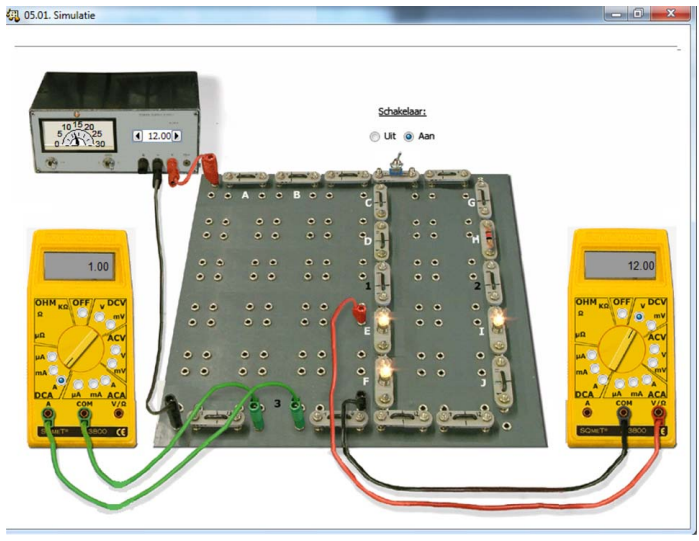
\includegraphics[scale=0.3]{images/chapter2/VirtualLab.png}
\caption{Image of the virtual-lab software}
\label{fig:image of the virtual-lab software}
\end{figure}

Two knowledge tests were used in this study, a prior knowledge test, and a post test. The tests were used to measure the learning outcomes of students. Both tests contained conceptual and procedural items. The conceptual items required the students to reason about the behavior of current and voltage in different circuits. The procedural items on the other hand handed participants a given circuit and required them to calculate the value of a specific variable.

\newpage
\subsubsection*{\underline{The results}}
\begin{table}[!ht]
    \caption{posttest results of the Traditional condition students}  
    \centering
    \begin{tabular}{|c|c|c|c|c|}
       \hline
         & M & S.D & Min & Max \\
       \hline
       Conceptual test (max. 14) & 4.09 & 1.83 & 1 & 9 \\
      \hline
       Procedural test (max. 5) & 2.96 & 0.93 & 1 & 5 \\
       \hline
       Total (max. 19) & 7.04 & 1.82 & 4 & 12 \\
       \hline
       \end{tabular}
    \label{tab:3}
\end{table}
\begin{table}[!ht]
    \caption{posttest results of the Virtual-lab condition students}  
    \centering
    \begin{tabular}{|c|c|c|c|c|}
       \hline
         & M & S.D & Min & Max \\
       \hline
       Conceptual test (max. 14) & 5.35 & 2.03 & 1 & 8 \\
      \hline
       Procedural test (max. 5) & 3.65 & 0.88 & 2 & 5 \\
       \hline
       Total (max. 19) & 9.00 & 2.20 & 5 & 12 \\
       \hline
       \end{tabular}
    \label{tab:4}
\end{table}

The test results show that the virtual-lab condition students obtained significantly higher overall scores, than the participants in the traditional condition. Virtual-lab students also scored higher on the conceptual items.

\subsubsection*{\underline{Conclusion}}
Posttest results showed that the virtual-lab students significantly outperformed the traditional students, and that can be observed in both the conceptual skills and the procedural skills. Virtual-lab students were also able to solve more complex problems than their traditional counterparts. It is worth mentioning however that the researchers did not replace practical laboratory activities with the virtual-lab, instead they gave students additional experiences using the virtual-lab software. That is because handling real equipment in the lab is also very necessary.

Finally, based on the previous findings, the researchers suggest that the best for the most benefit, virtual-lab software or inquiry-learning based methods in general should be a part of the students' experience when learning about electric circuits, in addition to their textbooks and practical lab activities \cite{25}.

\subsection{Gamification (in education) literature review}

\subsubsection{A Gamification Experience in a Class of a Degree in Engineering. (Ana Júlia Viamonte , 2018)}

Gamification as a learning strategy is increasingly discussed in the educational field. It offers a way for engaging and interactive learning making the educational content easily remembered and recalled. Ana Júlia noticed the lack of implementing gamification strategies in higher education. So she started this experiment where gamification strategies were used with the purpose of reducing the school dropout and increasing motivation to achieve better learning and higher passing rate especially with the first year of engineering courses  where a large group of students do not attend math classes which leads to higher failure rates.

\subsubsection*{\underline{Methodology:}}
The implementation of gamification started by replacing the evaluation with points that were collected by students for completing the evaluation components and for their participation in classes online. Students who have become players work to collect points and receive medals, avoid bombs and getting high scores to join the leaderboard.

The students earned experience points for completing a lesson or doing extra research which allowed them to get access to special powers. The special powers allowed the students to eliminate incorrect alternatives from a math test or  gain extra lives.if they had enough \acrshort{xp} they could buy help on tests. The students who barely registered in the course had a hundred of starting points and everything they did or didn't  was giving or taking points from them. There were twenty levels where each hundred points represented a level and the levels were corresponding to grades from zero to twenty.

The medals were reward attributes for performing certain tasks while the bombs were penalty attributes for not preforming certain tasks. 

The tests had three difficulty levels: easy, medium and hard. During the semester the students had to do six tests in moodle and to at least one level of each level. With the ability for the students to adjust the difficulty level, earning rewards from passing harder levels and doing extra work, With gamification the tests and exams turned into fighting against enemies and the class work turned into missions which allowed the students to increase their points reaching them to maximum. With this methodology the experiment started.

\subsubsection*{\underline{Results:}}

In this study the sample was the set of 294 students registered in the first year and first semester in electrotechnical engineering course, the majority were men only 7 \% of these students were women. 

With gamification the classes had a more challenging experience. There was a very large increase in the attendance numbers of each student. Traditionally in Math classes the attendance is low specially in first year but in that year the classes saw a considerable increase in attendance in both theoretical and practical classes and the rate of students who dropped out was lower than the previous years. See the figure below (figure \ref{fig:Students survey results}):
\begin{figure}[!ht]
     \centering
     \begin{subfigure}{0.4\textwidth}
         \centering
         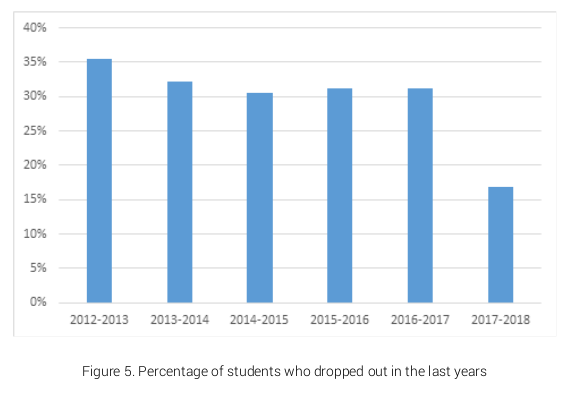
\includegraphics[width=\textwidth]{images/chapter2/image20.png}
         \caption{Percentage of students who dropped last year}
         \label{fig:Percentage of students who dropped last year}
     \end{subfigure}
     % \hfill
     \begin{subfigure}{0.4\textwidth}
         \centering
         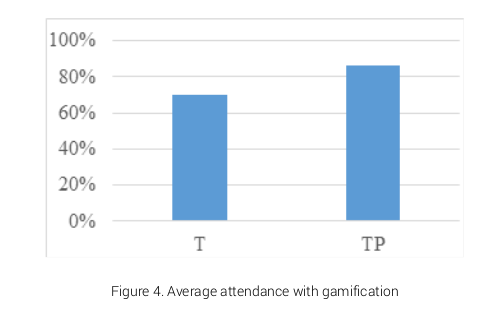
\includegraphics[width=\textwidth]{images/chapter2/image15.png}
         \caption{Average attendance with gamification}
         \label{fig:Average attendance with gamification}
     \end{subfigure}
        \caption{Students survey results}
        \label{fig:Students survey results}
\end{figure}

This experiment was reflected in the final approval rate as the students worked harder during the semester as they wanted to win the game, earning all medals and overcoming the challenges. The percentage of dropout of this course was very low (6\%) compared to previous years (15\% -30\%) the rate of failing was also low (33\%) 

\begin{figure}[!ht]
\centering
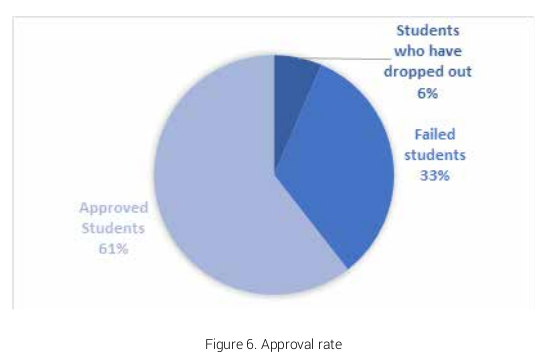
\includegraphics[scale=0.3]{images/chapter2/image18.png}
\caption{ Average rate}
\label{fig: Average rate}
\end{figure}
\newpage
A survey was made and the advantages and disadvantages were collected from the students showing as following:

\begin{table}[h!]
    \caption{Students Thoughts on the experiment}  
    \centering
    \begin{tabular}{|c|c|}
       \hline
       Advantages & Disadvantages \\
       \hline
       Motivation and stimulation of learning & Harder than previous year \\
       \hline
       Development of logical reasoning  & Over competitive \\ and problem-solving strategies and challenges. & \\
       \hline
       Competitiveness & Distractions with loss of focus of the content \\
       \hline
       Self-improvement and persistence. & Increased gambling addiction \\ 
       \hline
       Playful and dynamic way of learning & Mechanization: the student plays for \\ & playing and not for learning. \\
       \hline
       \end{tabular}
    \label{tab:5}
\end{table}

Of the students who answered 35\%  Considered the experiment to be excellent, 42\% very good , 20\% good and none of the students rated it as a bad or very bad experience.

\begin{figure}[!ht]
\centering
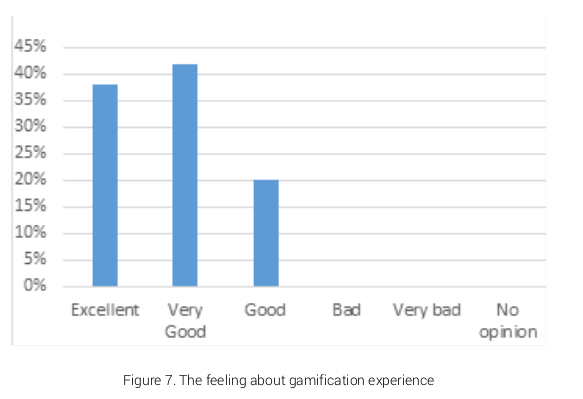
\includegraphics[scale=0.3]{images/chapter2/image14.png}
\caption{The feeling about Gamification on The experiment}
\label{The feeling about Gamification on The experiment
}
\end{figure}

The results of this research showed an educational success that year which illustrated How the games have a strong physical effect on people’s behavior. Making the gamification a valid approach to contribute to the students motivation prompting the students cognitive development. But the true potential of gamification is not easy to obtain as gamification may result in an unattractive and insufficient entertainment experience. That is why It is important to plan the educational objectives, discussing the strategies and analyzing the previous published experiences \cite{26}. 

\subsubsection{Electric Circuit Simulator Applying Augmented Reality and Gamification (Vinicio Burgos, César Guevara and Lorena Espinosa , 2021)}

\subsubsection*{\underline{Introduction}}

According to the statistics represented by Educational Evaluation National Institution (EENI) 22.8\% of the students form the Andean region and 18.3\% from the coast had insufficient grades in areas that include the study of science (Physics, Chemistry and Biology). From this point this Study proposes a solution by developing a physical mobile application That implements the methodologies of gamification and increased reality with the intention of improving creativity and academic performance of the students. The theme of this study focused on the implementing of direct current electric circuits. The proposed application will allow the students to learn and reinforce their knowledge continuously as the functionalities that will make up the application will consist of the ease of building different associations of electric circuits components putting the students in a competitive and challenging environment to solve problems and enhance their knowledge. 

\subsubsection*{\underline{Methodology}}

The learning circuits prototype was developed for the learning of electrical circuits in a series, parallel and mixed way consisting of an application that can be used from any device with data, fixed or mobile. There were countless limitations for carrying out this type of experiment in real laboratories. There is the fact that several institutions do not have the resources to implement them, adding to the risks of bad connections and the thermal effects that are generated or electrical shocks that could happen while experiencing electrical circuits in real life. 

The programmatic environment of “Scratch” was chosen to implement the application as it allows to carry out a block of programming in a synthetic, versatile, easily understood way for all users. See the figure \ref{fig:Scratch block programmatic environment, with application to the diagramming of electrical circuits}.

\begin{figure}[!ht]
\centering
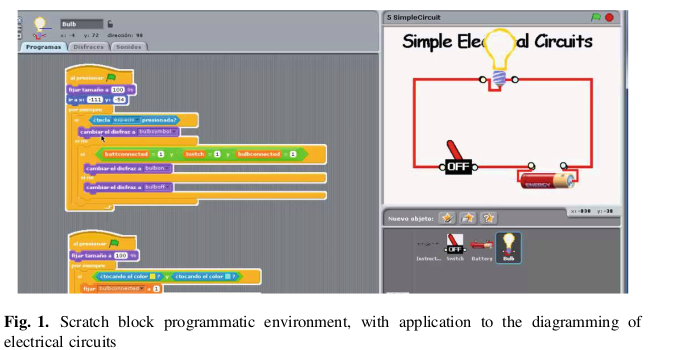
\includegraphics[scale=0.3]{images/chapter2/image4.png}
\caption{Scratch block programmatic environment, with application to the diagramming of electrical circuits}
\label{fig:Scratch block programmatic environment, with application to the diagramming of electrical circuits}
\end{figure}

The development of the circuit prototype included:
\begin{itemize}
    \item Defining the type and quantity of electrical devices that could be included
    \item Identifying  the connection  (parallel , serious or mixed).
    \item Considering the drawing of objects 
     how and will they interact.
     \item Including the necessary cables and switches, after which the blocks, sentences and appropriate coordinates.
     \item Declaring the variables and their condition within the chosen scenario.
     \item Programming of the electrical elements such as lights, LEDs and motors.
     \item Messages with their respective associated sound signals were included which identified as informative, motivational or safety alerts corresponding to danger or poorly connected circuits.
\end{itemize}

 \subsubsection*{\underline{Results}}

 The results that intended to be achieved from this proposal is improving the learning in circuits and increasing the motivation and creativity of the students leading to a significant advance in understanding the physical phenomenon of the subject leading to increasing the Academic performance of the students.

\subsubsection*{\underline{Conclusion}}

The Topic of electric circuits was selected Due to the large numbers of the students who have difficulties understanding how the electric circuits work and how the current flows through bulbs or any resistive elements. For this reason it is considered important and relevant to introduce this subject  in a fun , playful and entertaining way to achieve better understanding and to motivate students in this experimental science. The proposal shows a way for implementing electrical circuits including all the possibilities that give the students  to experiment and learn without the fear of risks that could happen while experimenting in the real world \cite{27}.
\newpage
\section{Case studies}
\subsection{Duolingo}

\begin{figure}[!ht]
\centering

\includegraphics[scale=0.05]{images/chapter2/image8.png}
\caption{case study subject logo (Duolingo)}
\label{case study subject logo (Duolingo)}
\end{figure}

More than two billion people worldwide are studying a foreign language (Forbes 2019), and digital learning seems to be on the rise for languages, with an estimated revenue around 6 billion dollars, and is expected to be 8.7 billion by 2025. But it's a vast market with lots of players around the globe, and the chance was there for a dominant one.

Duolingo already offers more languages than the competitors, they also include languages that aren’t spoken by lots of people, like Hawaiian. So it can always attract more users and new users can find the language they seek to learn. Along with offering more languages to learn, more users prefer duolingo because it’s free, compared with other competitors like Rosetta Stone which charges 120 dollars a year. Another competitor, Babble, has an estimated revenue of more that 115 million dollars from its yearly subscription fee of 85 dollars. 

\begin{figure}[!ht]
\centering
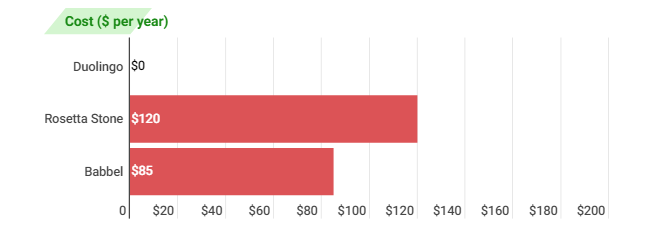
\includegraphics[scale=0.7]{images/chapter2/image9.png}
\caption{Duolingo versus competition: cost }
\label{Duolingo versus competition: cost }
\end{figure}

The huge popularity of duolingo isn’t just because it’s free of charge, that’s just one of its many advantages. The app is designed to grab the users and keep them engaged, using gamification elements and tricks, like points, badges, level system, treasure chests and streaks for continuous use of the app. Also, the app has a simple user interface designed to make it easy and effortless.
\newpage 
Duolingo’s three-minute lessons are designed to keep the learning experiment easy and approachable. Some of the disadvantages of using duolingo are that it doesn’t offer real world training, and that is a pivotal part when it comes to learning languages. Also, according to a study from 2020 some students find using the app boring, although the study also finds that most students disagree when it comes to the app being difficult to use or expensive, it still shows that there’s room to improve. \cite{28}\cite{29}

\begin{figure}[!ht]
\centering
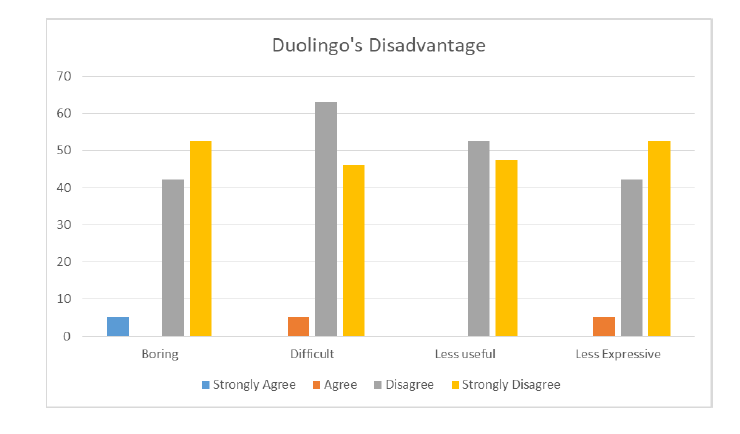
\includegraphics[scale=0.5]{images/chapter2/image21.png}
\caption{ Duolingo’s disadvantages based on a questionnaire}
\label{ Duolingo’s disadvantages based on a questionnaire }
\end{figure}
\newpage

\subsection{While True: Learn()}

\begin{figure}[h!]
\centering
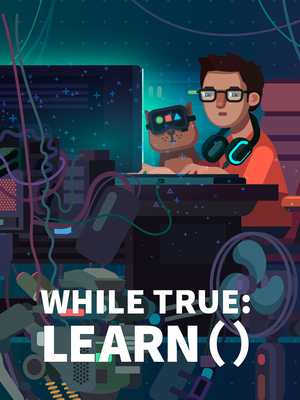
\includegraphics[scale=0.3]{images/chapter2/image12.jpg}
\caption{case study subject logo(While True: Learn())}
\label{ case study subject logo (While True: Learn())}
\end{figure}

Gamification in education can take many shapes and forms, \textit{While True: Learn()}, is more of a game than Duolingo and other educational applications. It teaches machine learning in a fun and easy way, whether you have advanced skills as a data scientist or not it doesn’t matter, anyone with basic knowledge of machine learning can play this game and learn a lot from that experience.  Throughout the game, users can learn the concept and principles of machine learning and programming gradually. The game has a low bar for beginners that doesn’t require them to be experts in the subject. Also, the game has shown from the get go that it has a high engagement rate with players.

With the release of the game, it has achieved more success than ever expected. Selling more than expected by the developers, and in different areas around the world, it had reached a wide variety of audience. Not only that, but at least three schools reported to have already started using the game in their educational process. Also, tech media coverage suggests that a large number of players have applied for machine learning courses and machine learning jobs after playing the game. There are huge advantages of playing this game, for starters you get to experience the concepts of machine learning at a very simplified level. Also, you get to try and learn from your mistakes while playing and try to better implement those concepts every time you play \cite{30}. 
\subsection{Quizlet}

\begin{figure}[!ht]
\centering

\includegraphics[scale=0.07]{images/chapter2/image5.png}
\caption{case study subject logo (Quizlet)}
\label{case study subject logo (Quizlet)}
\end{figure}

Much like duolingo, quiz let is an app that helps people to learn languages and test their knowledge of that language. Not only that, Quizlet will also help you learn about any subject in a large number of different fields. Its compact and easy-to-use practice material makes it fun and entertaining to learn about a new subject, whether it’s a new language, math, science or even game development. 

Quizlet offers a number of different options you can learn about a certain subject, flashcards, which can be used as a helpful memorization tool. Learn, write, spell, match are all different features and ways you can learn and test your knowledge. There’s also a “test” feature where you can answer questions based on the subject you ’ve been learning. A study has found that the majority of users spent around one hour weekly on the app, primarily using the “test” method. Some users spent more than three hours. Most of the users, though, didn’t like the “gravity” feature. 

Also in this study, we can tell that 95\% of users who have used Quizlet think it was a good tool for learning. And that’s not a new thing, because students will prefer a more gamified learning experience over the more traditional ones they find at schools. In addition, most students said that the friendly user interface of the app and the fact that they used different colors to distinguish different terms helps them remember those terms faster. 

When it comes to Quizlet’s disadvantages, all participants in the study reported that they can encounter some mistakes and errors. Due to the fact that any user can add lessons and publish it for other users to look up without evaluation. Also, most students have said that the app doesn’t show flexibility when it comes to the answers, meaning your answer isn’t correct unless it matches the answer put down by the one who designed those lessons. Although there’s some room for improvement, Quizlet shows that a gamified experience can capture the attention of students more than traditional learning methods. \cite{31}

\section{Project expected outcome and contributions}

Thus far, we’ve introduced the importance of \textit{electric circuit design}, the concepts of \textit{gamification} and \textit{game design}, and the problem with the state of electric circuit education (chapter 1), followed by a thorough literature review of gamification and electric-circuit-design-related research and projects. While there are some promising attempts at gamifying the electric circuit design learning experience, there are still many gaps to be filled (see 2.3); thus, this project’s expected outcome is \textbf{\textit{ to develop an educational puzzle game, whose player can both enjoy an entertaining experience regardless of their scientific interest level, all the while implicitly gaining valuable experience and knowledge in electric circuits design, where they can opt-in for a more academic learning experience through references to external materials, data-sheets, and circuit schematics designed to encourage real-life experimentation, and allow for academic instructors and supervisors to supplement their coursework and practical assignments with select (or all) sections of the game.}}

\subsection{Research contribution and future work}

From the research perspective, this project extends the current literature with a new perspective which more heavily employs the concepts of game design relative to previous gamification attempts. Future work may use all the source code and documents from this project to improve on one or more of the following aspects:
\begin{itemize}
    \item Apply other creative approaches and attempts at game design.
    \item Experiment with, and/or employ different approaches of gamification.
    \item Extend to a wider curricular scope.

\end{itemize}

\end{document}

 